\documentclass{article}
\usepackage{amsmath,amsthm,amssymb}
\usepackage {mathtext}
\usepackage{amsfonts} 
\usepackage[T1,T2A]{fontenc}
\usepackage[utf8]{inputenc}
\usepackage [english, russian] {babel}
\usepackage[babel=true]{microtype}
\usepackage{caption}
\usepackage{subcaption}
\captionsetup[table]{position=t,justification=raggedleft,slc=off}
\setlength{\abovecaptionskip}{0pt}
\usepackage {geometry}
\usepackage{graphicx}
\usepackage{multirow}
\geometry{margin=2cm}
\title{Отчёт о лабораторной работе №2.1.6. \\ Эффект Джоуля-Томсона}
\author{Павел Рудачихин \\ группа Б04-507}
\date{05.02.2026}
\begin {document}
\maketitle

\section* {Аннотация} 

\hspace{4mm}\textbf{Цель работы:} 1) определить изменения температуры углекислого газа при протекании через малопроницаемую перегородку при разных начальных значениях давления и температуры; 2) вычислить по результатам опытов коэффициенты a и b в модели Ван-дер-Ваальса.

\textbf{В работе используются:} трубка с пористой перегородкой, трубка Дьюара, жидкостный термостат ТЖ-ТС-01, дифференциальная термопара медь-константан, цифровой универсальный вольтметр В7-78/1, балластный баллон, манометр.

\textbf{Методы:} 1) определение  углового  коэффициента  наклона  зависимости двух величин; 2) измерение давления с помощью стрелочного манометра; 6) измерение напряжения с помощью цифрового вольтметра. 

\section* {Теоретические сведения}
\subsection*{Эффект Джоуля-Томсона}

\hspace{4mm} \textit{Эффектом Джоуля–Томсона} называется изменение температуры газа, медленно просачивающегося из области высокого в область низкого давления в условиях тепловой изоляции. В разрежённых газах,близких по свойствам к идеальным, при таком течении температура газа не меняется. Таким образом, в эффекте Джоуля–Томсона проявляется отличие исследуемого газа от идеального.

\begin{figure}[h!]
	\centering
	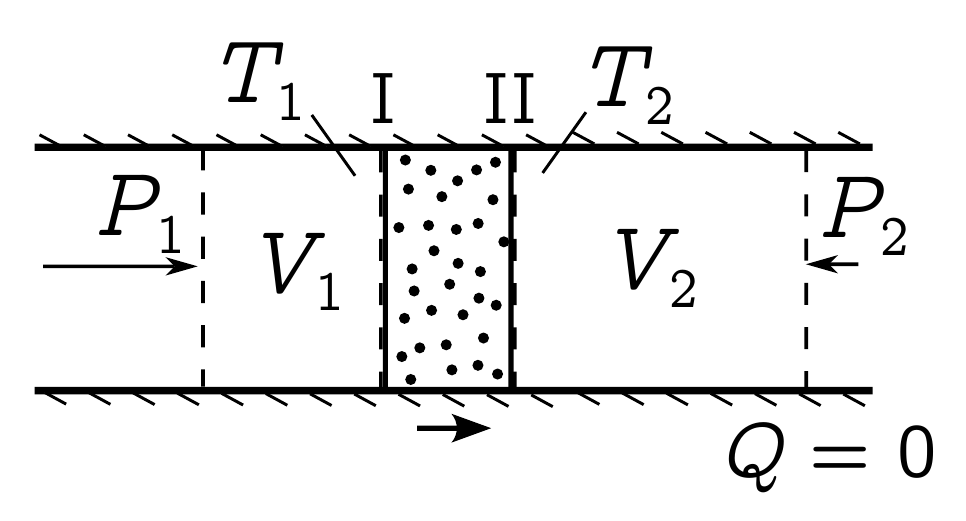
\includegraphics[width=0.6\linewidth]{1}
	\caption{Схема эффекта Джоуля-Томсона: трубка теплоизолирована $Q = 0$, газ из области повышенного давления $P_1$ проходит через пористую перегородку в область с атмосферным
		давлением $P_2$, $V_1$ и $V_2$ — молярные объёмы газа в сечениях I и II до перегородки и после неё соответственно, $T_1$ и $T_2$ — соответствующие температуры}
	\label{fig:1}
\end{figure}

Получим выражение для расчёта величины эффекта Джоуля–Томсона. Рассмотрим стационарный поток газа между сечениями I и II трубки до перегородки и после неё соответственно. Пусть через трубку прошёл $\Delta \nu = 1$ моль газа с молярной массой $\mu$. Пусть $V_1$ и $V_2$ — молярные объёмы газа в сечениях I и II, $P_1$ и $P_2$ — соответствующие давления, $U_1$ и $U_2$ — внутренние энергии в расчёте на 1 моль. Для того чтобы ввести в трубку порцию газа объёмом $V_1$, над ней нужно совершить работу $A'_1 = P_1 V_1$. Выходя через сечение II, эта же порция газа совершает работу $A_2 = P_2 V_2$. Так как трубка изолирована:

\begin{equation}
	A'_1 - A_2 = P_1 V_1 - P_2 V_2 = (U_2 + \mu v_2^2/2) - (U_1 + \mu v_1^2/2), 
\end{equation}

где кроме изменения внутренней энергии $U$ учтена кинетическая энергия течения $\mu v_1^2/2$. Определим \textit{молярную энтальпию} газа $H := U + PV$. Тогда уравнение (1) можно переписать как

\begin{equation}
H_1 - H_2 = \frac{\mu}{2}(v_2^2 - v_1^2). 
\end{equation}

Внутри пористой перегородки газ испытывает сильное трение. Это приводит к необратимому переходу почти всей кинетической энергии газа в тепловую. Поскольку система теплоизолирована, всё выделившееся тепло передаётся газу. Тогда закон сохранения энергии (2) остаётся в силе, однако его правая часть (кинетическая энергия) оказывается пренебрежимо малой. Тогда приходим к выводу, что эффект Джоуля–Томсона — это процесс, в котором сохраняется энтальпия:

\begin{equation}
H_1 \approx H_2.
\end{equation}

Энтальпия — функция состояния, зависящая как от температуры $T$, так и от давления $P$. Поэтому в результате просачивания газа под действием перепада давления $|\Delta P| = P_1 - P_2$ возникнет изменение его температуры $\Delta T = T_2 - T_1$. \textit{Коэффициентом Джоуля–Томсона} называют отношение

\begin{equation}
\mu_{\text{Д-Т}} = \frac{\Delta T}{\Delta P}. 
\end{equation}

Знак коэффициента Джоуля-Томсона может быть различным: он зависит как от сорта газа, так и от начальной температуры. Поскольку всегда $\Delta P < 0$, положительный $\mu_{\text{Д-Т}} > 0$ означает, что газ в процессе охлаждается. На практике эффект Джоуля–Томсона используют для получения низких температур методом дросселирования, поэтому понижение температуры принято считать «положительным» эффектом.

\subsection*{Вандерваальсова модель газа}

\hspace{4mm} Рассмотрим простейшую модель реального газа - газ Ван-дер-Ваальса. Термическое и калорическое уравнения состояния для него имеют следующий вид:

\begin{equation}
\left( P + \frac{a}{V^2} \right) (V - b) = RT,
\end{equation}
\begin{equation}
U = C_V T - \frac{a}{V}. 
\end{equation}

Константа $a$ отвечает за \textit{притяжение} молекул на дальних расстояниях, а константа $b$ отвечает за их \textit{отталкивание} при близком контакте и имеет смысл минимально возможного молярного объёма газа. 

Отсюда энтальпия газа Ван-дер-Ваальса:

\begin{equation}
H = U + PV = C_V T + RT \frac{V}{V-b} - \frac{2a}{V}. 
\end{equation}

Для упрощения формулы можно воспользоваться следующим обстоятельством: газ в опыте является достаточно разрежённым и довольно близок к идеальному. Поэтому его отличия от идеального следует учитывать только в эффекте Джоуля–Томсона, но не при вычислении объёма $V$. То есть, будем считать справедливой формулу (7), но объём в ней найдём из уравнения Менделеева–Клапейрона $V \approx RT/P$. Кроме того, можно положить $V \gg b$. В результате получим:

\begin{equation}
H \approx C_P T + P \left( b - \frac{2a}{RT} \right) 
\end{equation}

(здесь учтено также отношение Майера, что $C_V + R \approx C_P$).

Наконец, в качестве последнего упрощения примем, что относительное изменение температуры в опыте мало: $\Delta T/T \ll 1$. Тогда, полагая в этом приближении $\Delta H = 0$ для уравнения (8), получим окончательное выражение для коэффициента Джоуля–Томсона:

\begin{equation}
\mu_{\text{Д-Т}} = -\frac{\Delta T}{|\Delta P|} \approx \frac{\frac{2a}{RT} - b}{C_P}. 
\end{equation}


\subsection*{Температура инверсии}

\hspace{4mm} Из формулы (9) видно, что эффект Джоуля–Томсона зависит от соотношения параметров $a$ и $b$, которые оказывают противоположное влияние на знак эффекта. Если силы притяжения между молекулами велики, то основную роль играет член, содержащий $a$, и газ при расширении охлаждается. В обратном случае, когда доминирует отталкивание, т.е. слагаемое $b$, газ нагревается. Видно также, что существует температура инверсии эффекта Джоуля–Томсона

\begin{equation}
T_{\text{инв}} = \frac{2a}{Rb}, 
\end{equation}

при прохождении через которую эффект меняет знак. Для используемого в работе углекислого газа температура инверсии $T_{\text{инв}} \sim 1500$ К (при $P \sim 1$ атм), и при комнатной температуре он будет охлаждаться.


\section*{Экспериментальная установка}

\begin{figure}[h!]
	\centering
	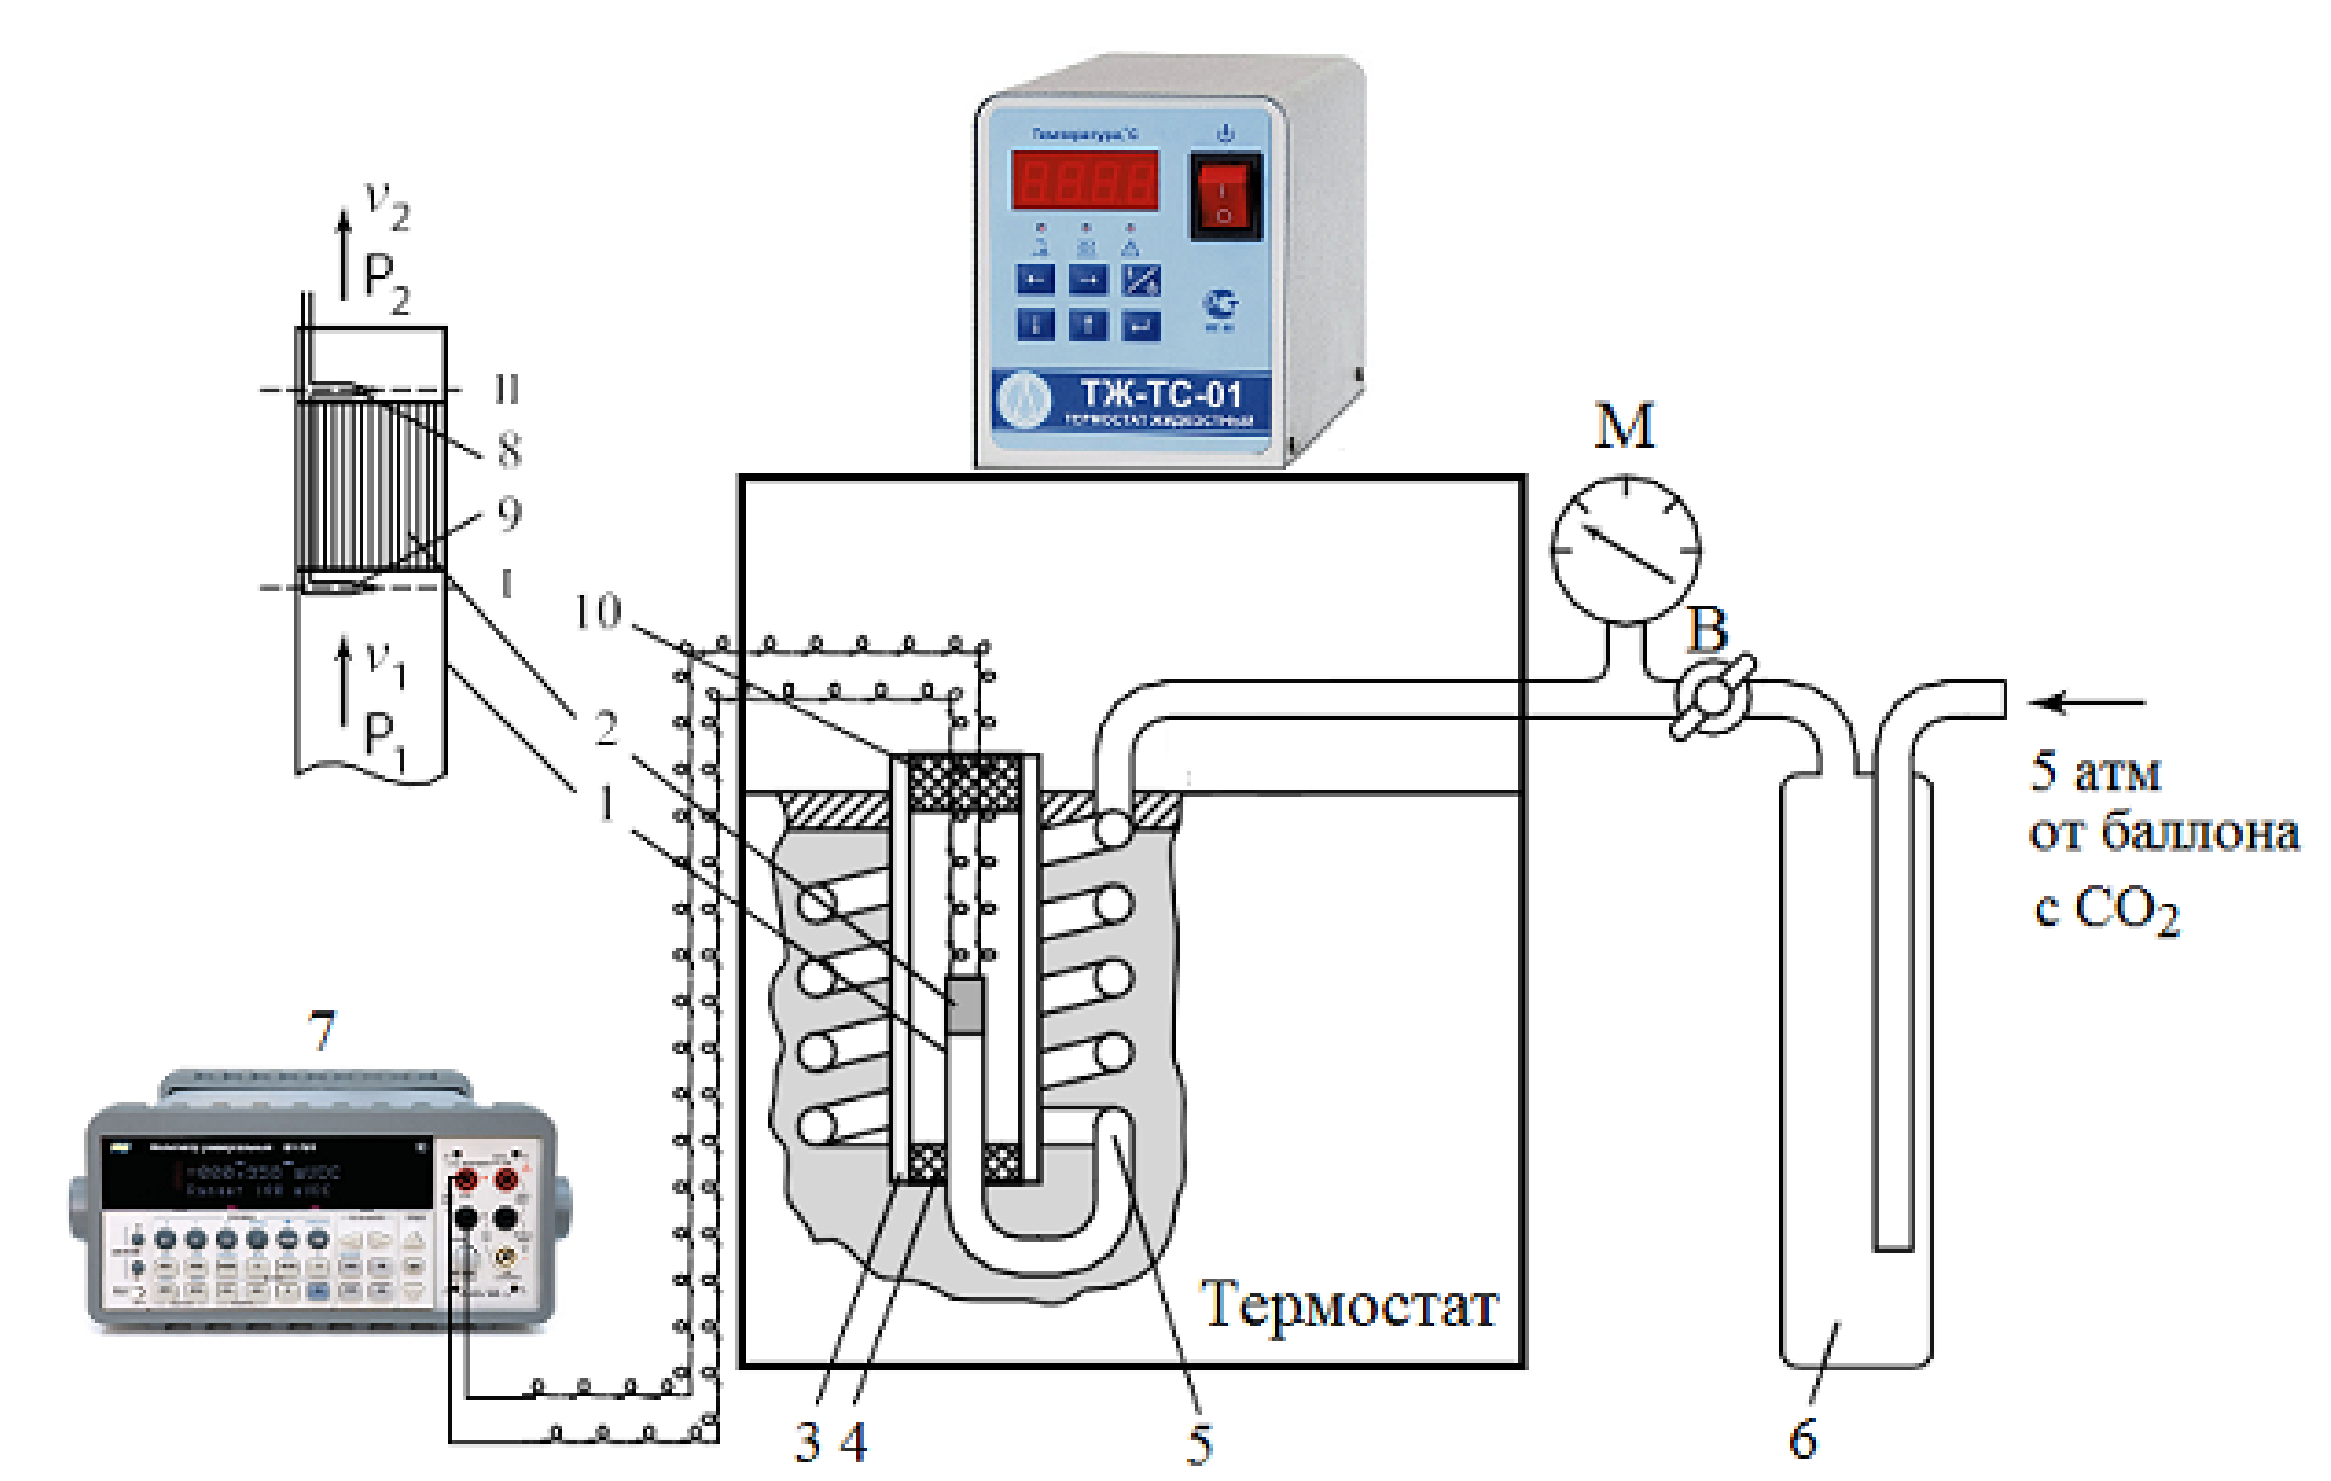
\includegraphics[width=0.7\linewidth]{2}
	\caption{Экспериментальная установка: 1 - трубка, 2 - пористая перегородка, 3 - труба Дьюара, 4 - уплотнительное кольцо, 5 - змеевик, 6 - балластный баллон, 7 - вольтметр, 8 и 9 - спаи термопары, 10 - пенопластовая пробка  М - манометр, В - вентиль}
	\label{fig:2}
\end{figure}



\hspace{4mm} Схема установки для исследования эффекта Джоуля–Томсона в углекислом газе представлена на рис. 2. Основным элементом установки является трубка 1 с пористой перегородкой 2, через которую пропускается исследуемый углекислый газ. Трубка имеет длину 80 мм и сделана из нержавеющей стали. Диаметр трубки $d = 3$ мм, толщина стенок 0,2 мм. \footnote{Гладун А.Д., Александров Д.А., Игошин Ф.Ф. и др. Лабораторный практикум по общей физике. М.: МФТИ, 2012.} Пористая перегородка расположена в конце трубки и представляет собой стеклянную пористую пробку со множеством узких и длинных каналов. Пористость и толщина пробки ($l = 5$ мм) подобраны так, чтобы обеспечить оптимальный поток газа при перепаде давлений $\Delta P \leq 4$ атм (расход газа составляет $Q \sim 10$ см$^3$/с); при этом в результате эффекта Джоуля–Томсона создаётся достаточная для надёжного измерения разность температур.

Углекислый газ под повышенным давлением поступает в трубку через змеевик 5 из балластного баллона 6. Медный змеевик омывается водой и нагревает медленно протекающий через него газ до температуры воды в термостате. Температура воды измеряется встроенным в термостат термометром. Термостат снабжён автоматическим терморегулятором, поддерживающим температуру воды с точностью $\pm 0,1^\circ$С.

Давление газа в трубке измеряется манометром М и регулируется вентилем В. Манометр М измеряет разность между давлением внутри трубки и наружным (атмосферным) давлением. Так как углекислый газ после пористой перегородки выходит в область с атмосферным давлением $P_2 = P_A$, этот манометр непосредственно измеряет перепад давления на входе и на выходе трубки $|\Delta P| = P_1 - P_2$.

Разность температур газа до и после перегородки измеряется дифференциальной термопарой медь–константан. Константановая проволока диаметром 0,1 мм соединяет спаи 8 и 9, а медные проволоки (того же диаметра) подсоединены к универсальному цифровому вольтметру 7. Отвод тепла через проволоку столь малого сечения пренебрежимо мал. Для уменьшения теплоотвода трубка с пористой перегородкой помещена в трубу Дьюара 3, стенки которой посеребрены для уменьшения теплоотдачи излучением. Для уменьшения теплоотдачи за счёт конвекции один конец трубы Дьюара уплотнён кольцом 4, а другой закрыт пробкой 10 из пенопласта. Такая пробка практически не создаёт перепада давлений между внутренней полостью трубы и атмосферой.

\section* {Методика измерений}
\subsection*{Измерение температуры}

Если спаи термопары помещены в точки с разными температурами, в её цепи возникает разность потенциалов $V$, которая и измеряется вольтметром. Зависимость $V(t)$ является, строго говоря, нелинейной, поэтому для восстановления температуры, как правило, необходимо использовать экспериментально полученные градуировочные кривые. В нашей работе измеряются малые перепады температуры, поэтому удобно использовать чувствительность термопары, т.е. наклон зависимости напряжения от температуры рабочего спая $dV/dt$. Тогда изменение $\Delta V$ связано с разностью температур спаев $\Delta t$ как $\Delta V \approx \frac{dV}{dt} \cdot \Delta t$. Чувствительность термопары зависит от температуры второго спая, т.е. в нашем случае — от температуры термостата. Соответствующие значения чувствительности для медно-константановой термопары приведены в табл. 1. 

\begin{table}[h!]
	\centering
	\captionbox{Чувствительность медно-константановой термопары}{
	\begin{tabular}{|c|c c c c c|}
		\hline
		Температура $t_0$, $^\circ$С & 0–10 & 10–20 & 20–30 & 30–40 & 40–50 \\
		
		Чувствительность $dV/dt$, мкВ/$^\circ$С & 39,1 & 39,8 & 40,7 & 41,5 & 42,4 \\
		\hline
		Температура $t_0$, $^\circ$С & 50–60 & 60–70 & 70–80 & 80–90 & 90–100 \\
		
		Чувствительность $dV/dt$, мкВ/$^\circ$С & 43,2 & 44,1 & 44,9 & 45,6 & 46,4 \\
		\hline
	\end{tabular}}
	\label{tab:1}
\end{table}


\section*{Используемое оборудование}

\hspace{4mm} В работе используется жидкостный \textbf{термостат} ТЖ-ТС-01. Погрешность определения температуры им составляет $\sigma_{\text{T}} = 0,1$ $^\circ$С

Погрешность стрелочного \textbf{манометра} определена ценой деления: $\sigma_{\text{P}} = 0,1$ бар.

Для измерения термоэдс использован цифровой универсальный \textbf{вольтметр} В7-78/1 на минимальном диапазоне 100 мВ. Погрешность вольтметра определена производителем так: 0,0035\% величины + 0,0005\% диапазона.


\section*{Результаты измерений}

\hspace{4mm} Измерения произведены для пяти значений давления при трёх значениях температур:

\begin{table}[h!]
	\centering
	\captionbox{Результаты измерений}{
	\begin{tabular}{|r|ccccc|}
		\hline
		Давление при $t = 21,1 ^\circ$С, бар &4,0       & 3,5       & 3,1       & 2,5       & 2,1 \\
		ЭДС, мкВ &153      & 127      & 110      & 83       & 64 \\
		\hline
		Давление при $t = 30,1 ^\circ$С, бар &4,0       & 3,5       & 3,0       & 2,5       & 2,0 \\
		ЭДС, мкВ &140      & 111      & 90       & 69       & 54 \\
		\hline
		Давление при $t = 50,0 ^\circ$С, бар &4,1       & 3,3       & 3,0       & 2,5       & 2,0 \\
		ЭДС, мкВ &105      & 77       & 66       & 47       & 31 \\
		\hline
	\end{tabular}}
\end{table}% 

\section*{Обработка результатов}
\subsection*{Оценка погрешностей}

\hspace{4mm} Обозначим чувствительность термопары $f$. Её погрешность составляет $\sigma_f = 0,3$ мкВ/$^\circ$С. \footnote{Гладун А.Д., Александров Д.А., Игошин Ф.Ф. и др. Лабораторный практикум по общей физике. М.: МФТИ, 2012.}

Разность температур спаев находим по формуле

\begin{equation}
	\Delta T = \frac{\Delta V }{f}
\end{equation}

Следовательно, погрешность этой разности определяем по известному правилу для независимых величин:

\begin{equation}
	\varepsilon_T^2 = \varepsilon_V^2 + \varepsilon_f^2
\end{equation}

где $\varepsilon$ означает относительную погрешность измерения. 

\subsection*{Построение графиков}

\begin{figure}[h!]
	\centering
	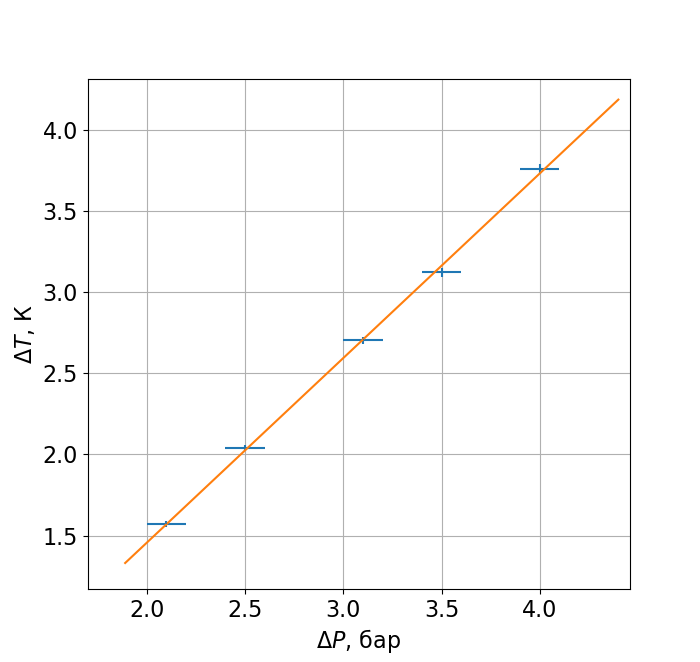
\includegraphics[width=0.45\linewidth]{F1}
	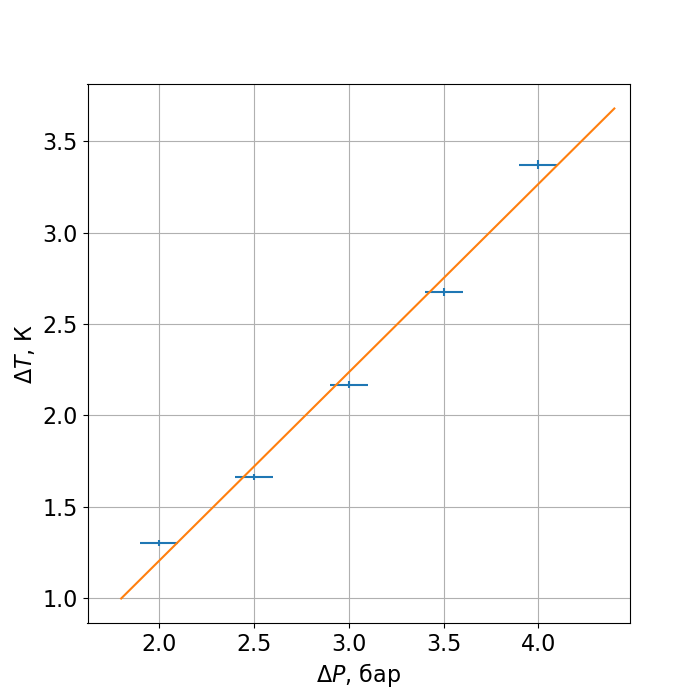
\includegraphics[width=0.45\linewidth]{F2}
	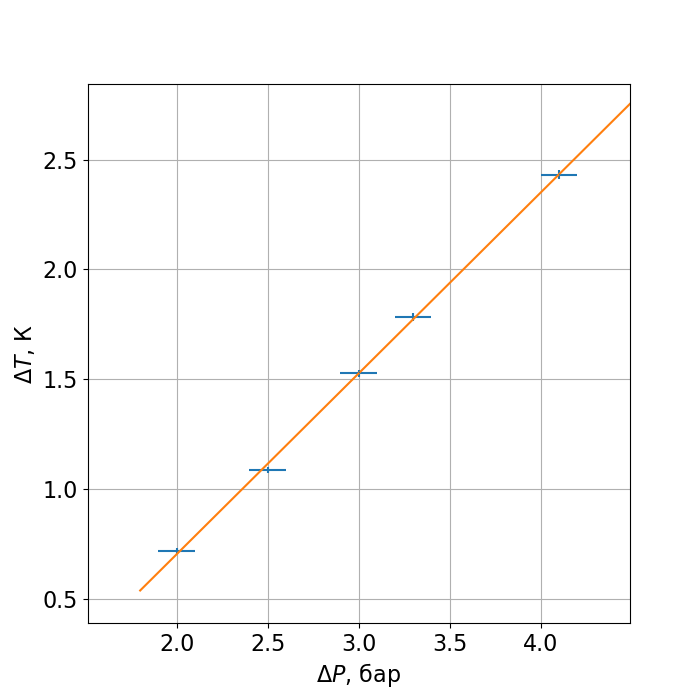
\includegraphics[width=0.45\linewidth]{F3}
	\caption{Графики зависимости $\Delta T (\Delta P)$ слева направо сверху вниз для $t_1 = 21,1 ^\circ$С, $t_2 = 30,1 ^\circ$С, $t_3 = 50,0 ^\circ$С}
	\label{fig:f1}
\end{figure}

\hspace{4mm} По формуле (11) из исходной зависимости $\Delta V (\Delta P)$ получаем искомую $\Delta T (\Delta P)$. Для всех трёх температур проводим лучшую прямую через имеющиеся точки (см. рис. 3) по методу наименьших квадратов:

\begin{equation}
	b = \frac{\langle xy \rangle - \langle x \rangle \langle y \rangle}{\langle x^{2} \rangle - \langle x \rangle^{2}} \ \ \ a = \langle y \rangle - b \langle x \rangle 
\end{equation}

где $a$ и $b$ - коэффициенты в уравнении прямой $y = bx + a$ . В нашем случае аргументом является $\Delta P$, а зависимой величиной $\Delta T$.

Погрешность этих коэффициентов (ошибка аппроксимации) определена так:

\begin{equation}
	\sigma_b \approx \dfrac{1}{\sqrt{n}}\sqrt{\frac{\langle y^2 \rangle - \langle y \rangle^2}{\langle x^{2} \rangle - \langle x \rangle^{2}} - b^2} \ \ \ \sigma_a = \sigma_b \sqrt{\langle x^{2} \rangle - \langle x \rangle^{2}}
\end{equation}

где $n$ - число измерений.

Все вычисления произведены с помощью написанной мною программы на языке Python (графики построены с помощью модуля Matplotlib). Получены следующие \textbf{значения коэффициента Джоуля-Томсона} (углового коэффициента прямой):

\begin{equation*}
	\boxed{\mu_1 = (1,136 \pm 0,016) \ К/бар, \ \ \mu_2 = (1,03 \pm 0,05) \ К/бар, \ \ \mu_3 = (0,823 \pm 0,009) \ К/бар}
\end{equation*}



\subsection*{Нахождение констант уравнения Ван-дер-Ваальса}

\hspace{4mm} Определим по формуле (9) константы уравнения Ван-дер-Ваальса. Запишем эту формулу так, чтобы явно показать линейную зависимость $\mu(1/T)$:

\begin{equation*}
	\mu = \frac{2a}{RC_P} \frac{1}{T} - \frac{b}{C_P} = A \cdot \frac{1}{T} - B
\end{equation*}

Решив систему из двух уравнений при разных значениях коэффициента Джоуля-Томсона и температур в общем виде, выразим $a$ и $b$:

\begin{equation*}
	a = \frac{R C_P}{2} \frac{\mu_1 - \mu_2}{1/T_1 - 1/T_2}
\end{equation*}

\begin{equation*}
	b = C_P \frac{\mu_1/T_2- \mu_2/T_1}{1/T_1 - 1/T_2}
\end{equation*}

Оказалось, что эти значения для двух пар температур почти не отличаются. Поэтому для их определения воспользуемся графическим методом (см. рис.4).

\begin{figure}[h!]
	\centering
	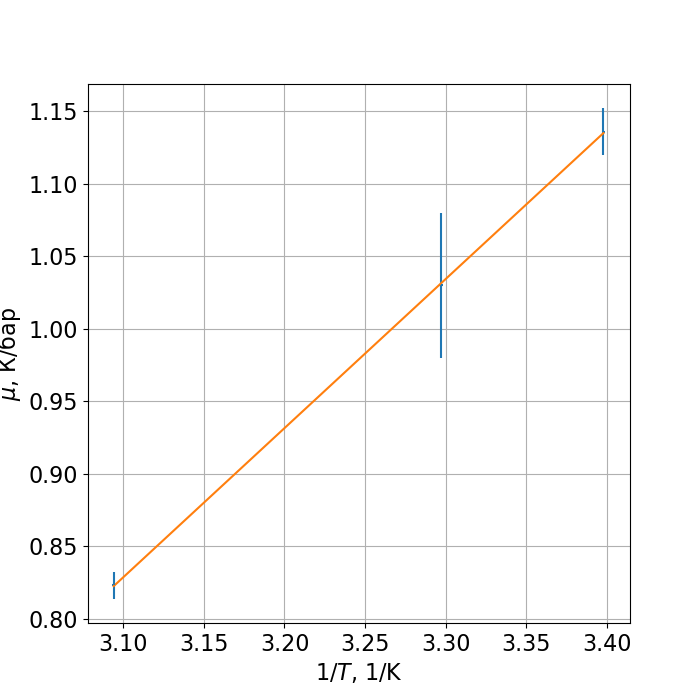
\includegraphics[width=0.5\linewidth]{F4}
	\caption{График зависимости $\mu (1/T)$ }
	\label{fig:f4}
\end{figure}

Аналогично определению коэффициента Джоуля-Томсона имеем:


\begin{equation*}
	A = (820 \pm 50) \ К^2/бар, \ \ \  B = (1,650 \pm 0,005) \ К/бар
\end{equation*}

В нашем диапазоне температур молярная теплоёмкость углекислого газа меняется мало, положим её $C_P = 37,1 \ Дж/моль \cdot К$ из справочника. Примем $R = 8,310 \ Дж/моль \cdot К$. Выразим коэффициенты уравнения Ван-дер-Ваальса:

\begin{equation*}
	a = 0,5 \cdot A R C_P  = (1,585 \pm 0,012) \ Н м^4/моль^2, \ \ \  b = B C_P = (186,5 \pm 0,9) \ см^3/моль
\end{equation*}

По формуле 10 определим температуру инверсии:

\begin{equation}
	T_{инв} = (2050 \pm 20) \ К
\end{equation}


\section*{Заключение}

\hspace{4mm} Значения коэффициентов Джоуля-Томсона согласуются со справочными данными. Однако значения констант уравнения Ван-дер-Ваальса завышены примерно в 4 раза. Вместе с тем температура инверсии совпадает со справочной в пределах погрешности, так как зависит от отношения констант, которое соответствует табличному. 

Причиной завышения констант $a$ и $b$ могли быть:

\begin{itemize}
	\item крайне малое количество экспериментальных данных, ибо по трём значениям невозможно установить зависимость с необходимой точностью;
	\item близость к критической температуре, что влияет на свойства газа;
	\item грубые приближения, например, разрежённость газа или теплоизоляция трубки.
\end{itemize}

Так или иначе, цели работы достигнуты: определено изменение температуры углекислого газа при протекании через малопроницаемую перегородку при разных начальных значениях давления и температуры; 2)по результатам опытов вычислены коэффициенты Джоуля-Томсона, константы a и b в модели Ван-дер-Ваальса.

\end {document}